\documentclass[9pt,twocolumn,twoside]{../../styles/osajnl}
\usepackage{fancyvrb}
\journal{i524} 

\title{Introduction to H2O}

\author[1]{Sushmita Sivaprasad}


\affil[1]{School of Informatics and Computing, Bloomington, IN 47408, U.S.A.}


\affil[*]{ sushsiva@umail.iu.edu}

\dates{\today}

\ociscodes{machine learning, data mining,predictive analytics,cloud}

% replace this with your url in github/gitlab
\doi{\url{https://github.com/SushmitaSivaprasad/sp17-i524/tree/master/paper1/S17-IR-2038/report.pdf}}


\begin{abstract}
  
Machine learning and data mining have been used everyday in all
industries driven by data. H2O is a platform using for performing
machine learning and predictive analytics for large scale date using
cloud. When the data that is generated is large scale and is in
terrabytes, H2O serves a very important purpose of being able to
accurately predict using different algorithms using different
programming languages through APIs. This paper introduces to H2O, how
this platform  has impacted various industries across several domains with
improved accuracy and reduced processing time. Different use cases of
the H2O platform has been explained as well.
  
\end{abstract}

\setboolean{displaycopyright}{true}

\begin{document}

\maketitle

\TODO{This review document is provided for you to achieve your
  best. We have listed a number of obvious opportunities for
  improvement. When improving it, please keep this copy untouched and
  instead focus on improving report.tex. The review does not include
  all possible improvement suggestions and for each comment you may
  want to check if it applies elsewhere in the document.}

\TODO{Abstract: There are some grammar issues that need to be
  addressed, otherwise looks good.}

\TODO{Your paper is a little short of the requirement and can be
  expanded a little bit.}

\TODO{Please, make sure you know how to use citations
  correctly. Citations go after the text that references them, and
  before any periods or other punctuation. In some instances you've
  just included them at the beginning of a whole paragraph, but a
  citation should be used for more specific statements in your paper.}

\TODO{Your paper gives a good overview of H2O, but certain sections
  can be expanded and/or clarified. The use cases can use more detail
  on what the actual outcomes were. See the specific notes below.}

\TODO{Assessment: Revisions required. Please address the review
  comments by end of March.}

\section{Introduction}

\cite{www-h2o-webpage}H2O \CE \TODO{The citations needs to go at the
  end of the text that references it.} is an open source platform that
is used to create machine learning and predictive analytics models on
big datasets. It is mainly written in Javascript but have APIs for R ,
Python, Excel, Tableau and Flow and works on the conventional
operation systems. \TODO{"conventional operating systems" is too
  vague. You either can omit OS information altogether since someone
  can check this in the docs easily, or give a better idea of what is
  supported. The first option is sufficient for an overview paper like
  this.} This platform allows the online scoring and modelling of data
on a single algorithm. \TODO{This is not worded very clearly. Do you
  mean that each algorithm provided can be evaluated separately? If
  so, this is too fine a detail for an overview and you can omit
  it. If not, please clarify.} The main algorithms implemented on the
datasets are deep learning, gradient boosting , generalized linear
model, distributed random forest, k-means etc. \TODO{With the "etc."
  it's not clear whether these are really the main algorithms, or just
  a subsection that you decided to list. This can be worded better.}
The algorithms implemented on the big datasets is read in a parallel
manner and is then distributed and stored in memory in a compressed
column format. H2O also has an inbuilt intelligence to detect and
support the data ingest \TE \TODO{data ingest?} from various sources
in different formats.

\section{How does H2O work?}

\cite{www-h2oyoutubevideo}H2O \CE is mainly used for large dataset ,
usually in the range of terrabytes. \TODO{Are there any drawbacks to
  using on smaller datasets?} A company might have their dataset
stored on big data systems such as hadoop. \TODO{Please, capitalize
  names like "Hadoop."} When we analyze a data \GE usually we choose a
smaller sample dataset rather than the entire dataset to build model
due to the large processing time involved. H2O has the advantage of
being able to use the entire dataset to run the algorithm on as larger
the dataset we are able to analyse better the predictions would
be. Suppose a business is trying to understand the best product
placement for optimal customer enagement, the model would be created
based on the dataset formed collecting information about the
interactions of the customer on the website. \GE H20 is used to model
all of the data with multiple algorithms using more than one machine
at the same time, this way we don’t have to sample the data to predict
for performance. \TODO{This is not quite true. There are reasons
  beyond performance you may want to sample your dataset or break it
  up into portions for training and testing your algorithms for
  example. In addition, some of the algorithms simply don't scale, and
  being implemented well in H20 or another parallel system still
  doesn't make them applicable to very large data.} H2O is also used
to score hundreds of models in nano seconds to reach better
predictions. \TODO{Nanoseconds is very specific. Do you have a
  citations for this?}

\section{Requirements}

\subsection{Operating Systems}
\cite{www-h2o-requirements}
It works on the following operating systems 
\newline Windows 7 or later
\newline OSX 10.9 or later
\newline Ubuntu 12.04
\newline RHEL/CentOS6 or later

\subsection{Languages}

 Java 7 or later
\newline Scala 2.10 or later
\newline R version 3 or later
\newline Python 2.7x or 3.5x
 
\subsection{Browser}

 Chrome
\newline Safari
\newline Internet Explorer
\newline Firefox

\subsection{Hadoop}
 Optional Cloudera CDH 5.2 or later
\newline MapR 3.1.1 or later
\newline Hortonworks HDP 2.1 or later

\TODO{This kind of detail is not necessary in an overview paper. Your
  goal is to give an overview so someone can decide if H2O is
  something they may be interested in. They can later consult the docs
  about specific system information like this.}

\section{Architecture}
\cite{www-h2o-architecture} The H2O architecture consists of a
different component \GE which combine together to form the H2O
software stack. We can divide the H2O architecture into 3 different
components, top section includes all the REST API clients, middle
includes the Network Cloud and the bottom section contains the
different components that run within an H20 JVM process. The top
section contains the programming languages that can be used on the big
dataset here. The REST API clients communicate with the H2O with the
help of a socket connection. The Network cloud consists of the
different inbuilt algorithms to create the necessary model on the
data, this can also contain a customized customer algorithm to analyze
the required dataset and produce the desired outputs.  The H2O cloud
can consists of two or more nodes which can contain a single JVM
process. \TODO{H2O being based on JVM is something you want to mention
  earlier and more prominently.} Each JVM process consists of
language, algorithm and infrastructure (manages the resources
management such as memory and CPU).

\section{Figures}

\begin{figure}[htbp]
\centering
\fbox{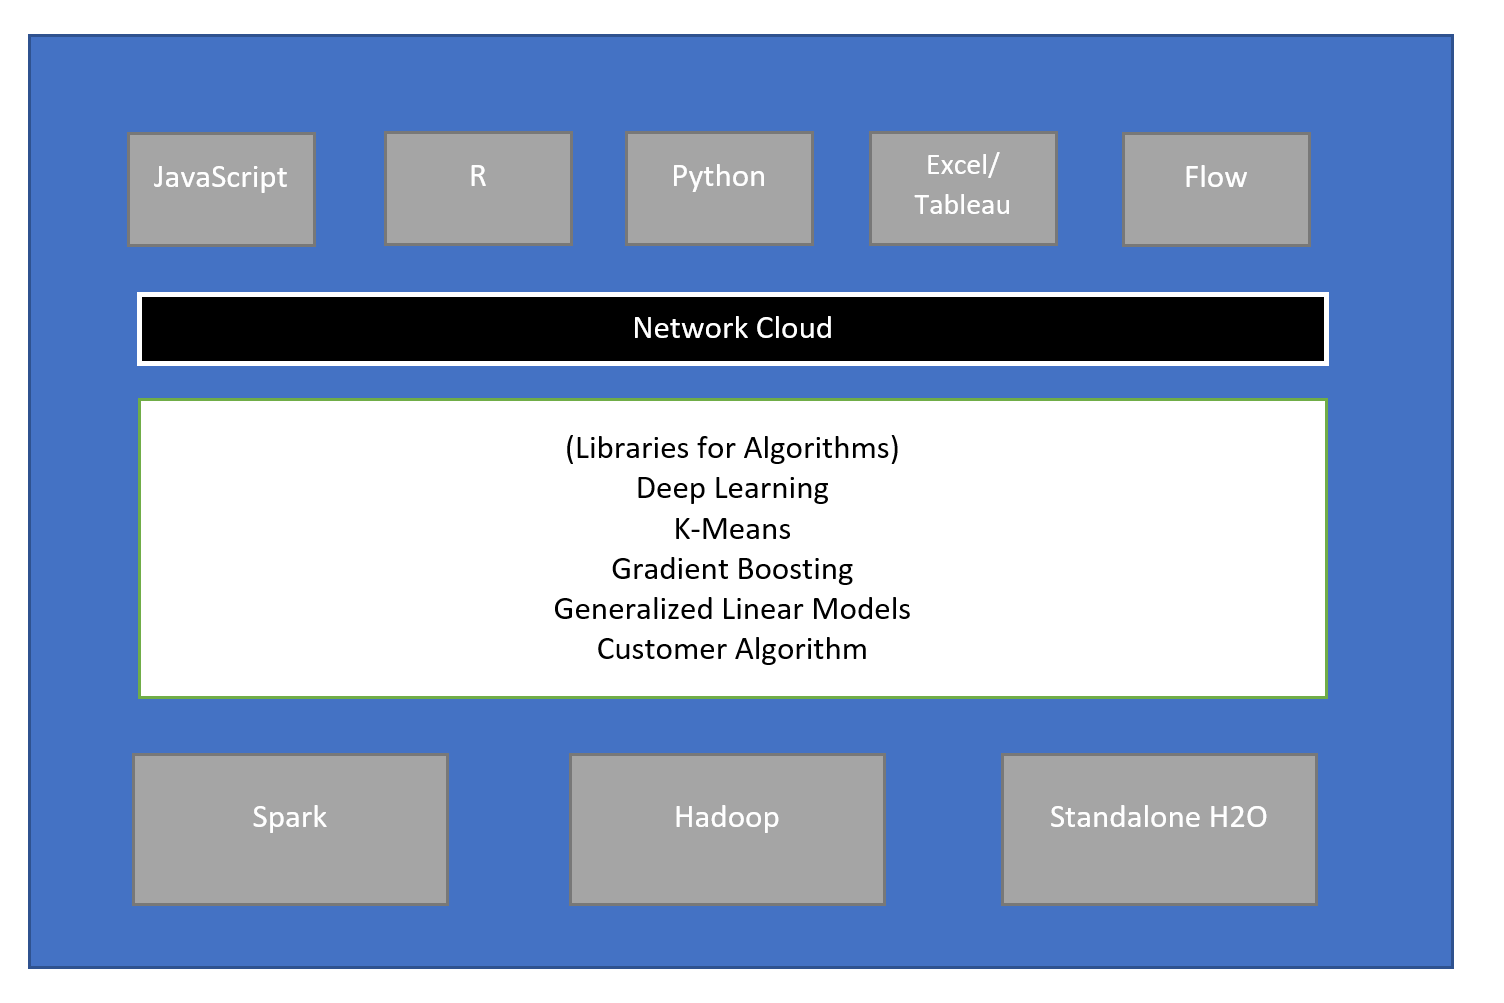
\includegraphics[width=\linewidth]{images/Architecture(1)}}
\caption{H2O Architecture\cite{www-h2o-architecture}}
\label{ fig:Architecture of H2O}
\end{figure}


\section {Used Cases}

\subsection { CapitalOne}
\cite{www-h2o-capitalone} \CE CapitalOne, a fortune 500 bank with 960
banks and 2000 ATMs accumulates terrabytes of information in real time
on customer information and financial processing. H2O was used to
reduce the iterative timing \TODO{I am not sure what "iterative
  timing" refers to here. Please elaborate.} over the large data sets
on applying various algorithms. Different algorithms can be applied to
find which one works best due to reduction in time consumed in
processing these large datasets. A large number of hard and soft
metrics were evaluated as well using machine learning frameworks.

\TODO{It's not clear from this paragraph what CapitalOne actually used
  H2O for. What did they analyze and what did they find? Or how are
  they applying the algorithms to their real-time data?}

\subsection {MarketShare}
\cite{www-h2o-marketshare} The company MarketShare have implemented
H2O to optimize budgeting for marketing. Since marketing approaches
are data driven features , predictive analytics under H2O was used to
give a comparison on how the current state of the marketing budget is
and how much is the predicted revenue, using H2O solutions were
generated as to what are the changes that can be made to improve the
current projection and what an improved projection will look
like. \TODO{This was a very long sentence. It will be more clear and
  easier to read if you break it up.} H2O can ingest large amount of
data as its capability is not limited to using one machine , since it
is a cloud based system, multiple machines can be used at the same
time. \TODO{This is information you already went over earlier and
  doesn't need to be restated here.} MarketShare was able to go on the
cloud and use as much machines as required and get desired outputs on
the large datasets. They use 25 machines for all of their clients to
process the data and were able to expand the scalability of the
dataset.If their datasize increases by x amount then they would add y
more machines to solve the problem. Scaling across lot of nodes is
critical to their business as the company deals with digital log data
and irrespective of the complexity of the modelling and the huge size
of the data. It has a distributed in-memory processing with the kind
of data involved and the algorithms implemented on the
data. \TODO{Like before, this is information about H2O you already
  went over.}

\TODO{It would be helpful to find what the outcomes for MarketShare
  were when using H2O. Did their marketing yield better results when
  using H2O?}

\section {Relevant Coursework}
\TODO{Better use "resources" than "coursework"}

H2O has an open source platform and hence has a community for
support.\newline Step by step instructions with documentation and
videos have been provided for installation and to understand the work
flow of H2O.\newline Free online training videos are provided on the
main webpage \cite{www-h2o-learn} \newline H2O documentation is
available on their website.  \cite{www-h2o-webpage}\newline h2ostream
is an open source google group where H2O users can post questions and
get answers.\newline They have built an online community
at\cite{www-h2o-community} which is a discussion platform.\newline
They also conduct conferences around the year in United States for
users to interact among one another and update new releases and
happenings in the big data community.\cite{www-h2o-meetups}

\TODO{You shouldn't use the \emph{newline} command like this. You can
  either use paragraphs or bullet points. This kind of formatting is
  very unusual.}

\section{Conclusion}
\cite{www-h2o-why} \CE Being an open source platform it gives user the
flexibility to solve the problems. It is easy to set up and has a
smooth installation and usage feature due to its interface with
familiar programming environments using APIs. Models can also be
inspected during training.It can ingest \TE any format of file , it
can even connect to data from HDFS, S3 ,SQL and NoSQL data sources.It
has a massive \TODO{"massive" is subjective, please avoid}
scalability, large datasets can be analyzed by using multiple
machines. It also conducts a real time data scoring for accurate
predictions.

\section{Acknowledgement}
A very special thanks to Professor Gregor von Laszewski and the
teaching assistants Miao Zang and Dimitar Nikolov for all the support
and guidance in getting this paper done and resolving all the
technical issues faced. The paper is written during the spring 2017
semester course {I524: Big Data and Open Source Software Projects} at
Indiana University Bloomington.

\bibliography{references}

\end{document}
